% Autor: Alex Oster, Jonathan Sigrist, Luca Wiggering
% Datum: 2018-01
% basiert auf der Vorlage für Versuchsprotokolle von Simon May

%\includeonly{
%	tex/04_Titelseite,
%	tex/05_Gliederung,
%	tex/14_Kurzfassung,
%	tex/15_Theorie,
%	tex/16_Methoden,
%	tex/17_Ergebnisse,
%	tex/19_Zusammenfassung,
%	tex/20_Anhang,
%	tex/21_Literatur
%}

\documentclass[
	a4paper,                % Papierformat (DIN A4)
	titlepage=firstiscover, % Separate Titelseite
	captions=tableheading,  % \caption bei Tabellen immer als Überschrift setzen
	toc=bibliography,       % Literaturverzeichnis im Inhaltsverzeichnis aufführen
	toc=listof,             % Abbildungsverzeichnis etc. im Inhaltsverzeichnis aufführen
	oneside,                % Einseitig
	%twoside,               % Zweiseitig
	%twocolumn,             % Zweispaltig
	automark,               % Abschnittstitel automatisch in Kopfzeile einfügen
	12pt,                   % Schriftgröße (beliebige Größen mit „fontsize=Xpt“)
	english, ngerman,		% Sprache für z.B. Babel; ausgewählt: ngerman (letztgenannt)
	%draft=true             % Entwurf-Modus; markiert zu lange und zu kurze Zeilen
]{scrartcl}

% Autor: Simon May
% Datum: 2017-10-04

% --- Pakete einbinden
% --- Pakete erweitern LaTeX um zusätzliche Funktionen.
%     Dies ist ein Satz nützlicher Pakete.

% Silbentrennung etc.; Sprache wird durch Option bei \documentclass festgelegt
\usepackage{babel}
\usepackage{iftex}
\ifLuaTeX
	% Schriftart (Latin Modern)
	\usepackage{fontspec}
	\fontspec{Latin Modern Roman}
\else
	% Verwendung der Zeichentabelle T1 (für Sonderzeichen etc.)
	\usepackage[T1]{fontenc}
	% Legt die Eingabe-Zeichenkodierung fest, z.B. UTF-8
	\usepackage[utf8]{inputenc}
	% Schriftart (Latin Modern)
	\usepackage{lmodern}
	% Zusätzliche Sonderzeichen
	\usepackage{textcomp}
\fi

\usepackage{upgreek}
% Nutzen von +, -, *, / in \setlength u.ä. (z.B. \setlength{\a + 3cm})
\usepackage{calc}
% Wird benötigt, um \ifthenelse zu benutzen
\usepackage{xifthen}
% Optionen für eigene definierte Befehle
\usepackage{xparse}

% Verbessertes Aussehen des Schriftbilds durch kleine Anpassungen
\usepackage{microtype}
% Automatische Formatierung von Daten
\usepackage[useregional]{datetime2}
% Wird für Kopf- und Fußzeile benötigt
\usepackage{scrlayer-scrpage}
% Einfaches Wechseln zwischen unterschiedlichen Zeilenabständen
\usepackage{setspace}
% Optionen für Listen (enumerate, itemize, …)
\usepackage{enumitem}
% Automatische Anführungszeichen
\usepackage{csquotes}
% Zusätzliche Optionen für Tabellen (tabular)
\usepackage{array}

% Mathepaket (intlimits: Grenzen über/unter Integralzeichen)
\usepackage[intlimits]{amsmath}
% Mathe-Symbole, \mathbb etc.
\usepackage{amssymb}
% Weitere Mathebefehle
\usepackage{mathtools}
% „Schöne“ Brüche im Fließtext
\usepackage{xfrac}
% Ermöglicht die Nutzung von \SI{Zahl}{Einheit} u.a.
\usepackage{siunitx}
% Ermöglicht Nutzung von \pdv als Ableitungen
\usepackage{physics}
% Definition von Unicode-Symbolen; Nach [utf8]inputenc laden!
\usepackage{newunicodechar}
% Unicode-Formeln mit pdfLaTeX
% Autor: Simon May
% Datum: 2015-03-04

% Diese Datei ermöglicht es, Mathe-Symbole (z.B. \gamma) direkt als
% Sonderzeichen (d.h. γ) einzugeben

% silence unterdrückt Warnungen; vor hyperref laden
\usepackage{silence}
\WarningFilter[pdflatex-unicode-math]{newunicodechar}{Redefining Unicode character}
\ActivateWarningFilters[pdflatex-unicode-math]

\newunicodechar{†}{\dag}
\newunicodechar{‡}{\ddag}
\newunicodechar{…}{\ldots}
\newunicodechar{⋯}{\cdots}
\newunicodechar{⋮}{\vdots}
\newunicodechar{⋱}{\ddots}
\newunicodechar{⋰}{\iddots}
\newunicodechar{α}{\alpha}
\newunicodechar{β}{\beta}
\newunicodechar{γ}{\gamma}
\newunicodechar{δ}{\delta}
\newunicodechar{ε}{\varepsilon}
\newunicodechar{ϵ}{\epsilon}
\newunicodechar{ζ}{\zeta}
\newunicodechar{η}{\eta}
\newunicodechar{θ}{\theta}
\newunicodechar{ϑ}{\vartheta}
\newunicodechar{ι}{\iota}
\newunicodechar{κ}{\kappa}
\newunicodechar{ϰ}{\varkappa}
\newunicodechar{λ}{\lambda}
\newunicodechar{μ}{\mu}
\newunicodechar{ν}{\nu}
\newunicodechar{ξ}{\xi}
\newunicodechar{ο}{o}
\newunicodechar{π}{\pi}
\newunicodechar{ρ}{\rho}
\newunicodechar{ϱ}{\varrho}
\newunicodechar{σ}{\sigma}
\newunicodechar{τ}{\tau}
\newunicodechar{υ}{\upsilon}
\newunicodechar{φ}{\varphi}
\newunicodechar{ϕ}{\phi}
\newunicodechar{χ}{\chi}
\newunicodechar{ψ}{\psi}
\newunicodechar{ω}{\omega}
\newunicodechar{Α}{\mathrm{A}}
\newunicodechar{Β}{\mathrm{B}}
\newunicodechar{Γ}{\Gamma}
\newunicodechar{Δ}{\Delta}
\newunicodechar{Ε}{\mathrm{E}}
\newunicodechar{Ζ}{\mathrm{Z}}
\newunicodechar{Η}{\mathrm{H}}
\newunicodechar{Θ}{\Theta}
\newunicodechar{Ι}{\mathrm{I}}
\newunicodechar{Κ}{\mathrm{K}}
\newunicodechar{Λ}{\Lambda}
\newunicodechar{Μ}{\mathrm{M}}
\newunicodechar{Ν}{\mathrm{N}}
\newunicodechar{Ξ}{\Xi}
\newunicodechar{Ο}{\mathrm{O}}
\newunicodechar{Π}{\Pi}
\newunicodechar{Ρ}{\mathrm{P}}
\newunicodechar{Σ}{\Sigma}
\newunicodechar{Τ}{\mathrm{T}}
\newunicodechar{Υ}{\Upsilon}
\newunicodechar{Φ}{\Phi}
\newunicodechar{Χ}{\Chi}
\newunicodechar{Ψ}{\Psi}
\newunicodechar{Ω}{\Omega}
\newunicodechar{∑}{\sum}
\newunicodechar{∫}{\int}
\newunicodechar{∬}{\iint}
\newunicodechar{∭}{\iiint}
\newunicodechar{⨌}{\iiiint}
\newunicodechar{∮}{\oint}
\newunicodechar{∯}{\oiint}
\newunicodechar{∰}{\oiiint}
\newunicodechar{∇}{\nabla}
\newunicodechar{∂}{\partial}
\newunicodechar{√}{\sqrt}
\newunicodechar{∈}{\in}
\newunicodechar{∋}{\ni}
\newunicodechar{∉}{\notin}
\newunicodechar{∀}{\forall}
\newunicodechar{∃}{\exists}
\newunicodechar{∄}{\nexists}
\newunicodechar{∴}{\therefore}
\newunicodechar{∵}{\because}
\newunicodechar{〈}{\langle}
\newunicodechar{〉}{\rangle}
\newunicodechar{⌊}{\lfloor}
\newunicodechar{⌋}{\rfloor}
\newunicodechar{⌈}{\lceil}
\newunicodechar{⌉}{\rceil}
\newunicodechar{∼}{\sim}
\newunicodechar{∝}{\propto}
\newunicodechar{∞}{\infty}
\newunicodechar{ℵ}{\aleph}
\newunicodechar{ℏ}{\hbar}
\newunicodechar{℘}{\wp}
\newunicodechar{ℓ}{\ell}
\newunicodechar{∅}{\emptyset}
\newunicodechar{×}{\times}
\newunicodechar{⋅}{\cdot}
\newunicodechar{÷}{\div}
\newunicodechar{⋆}{\star}
\newunicodechar{∘}{\circ}
\newunicodechar{⋄}{\diamond}
\newunicodechar{⊕}{\oplus}
\newunicodechar{⊖}{\ominus}
\newunicodechar{⊗}{\otimes}
\newunicodechar{⊘}{\oslash}
\newunicodechar{⊙}{\odot}
\newunicodechar{±}{\pm}
\newunicodechar{∓}{\mp}
\newunicodechar{≈}{\approx}
\newunicodechar{≡}{\equiv}
\newunicodechar{≠}{\ne}
\newunicodechar{≥}{\ge}
\newunicodechar{≤}{\le}
\newunicodechar{≫}{\gg}
\newunicodechar{≪}{\ll}
\newunicodechar{⊂}{\subset}
\newunicodechar{⊃}{\supset}
\newunicodechar{⊆}{\subseteq}
\newunicodechar{⊇}{\supseteq}
\newunicodechar{⊈}{\nsubseteq}
\newunicodechar{⊉}{\nsupseteq}
\newunicodechar{≔}{\coloneqq}
\newunicodechar{≕}{\eqqcolon}
\newunicodechar{¬}{\neg}
\newunicodechar{∨}{\vee}
\newunicodechar{∧}{\wedge}
\newunicodechar{∪}{\cup}
\newunicodechar{∩}{\cap}
\newunicodechar{⋁}{\bigvee}
\newunicodechar{⋀}{\bigwedge}
\newunicodechar{⋃}{\bigcup}
\newunicodechar{⋂}{\bigcap}
\newunicodechar{⟂}{\perp}
\newunicodechar{∥}{\parallel}
\newunicodechar{∦}{\nparallel}
\newunicodechar{𝚤}{\imath}
\newunicodechar{𝚥}{\jmath}
\newunicodechar{⇔}{\Leftrightarrow}
\newunicodechar{⇕}{\Updownarrow}
\newunicodechar{⇐}{\Leftarrow}
\newunicodechar{⇒}{\Rightarrow}
\newunicodechar{⇑}{\Uparrow}
\newunicodechar{⇓}{\Downarrow}
\newunicodechar{↔}{\leftrightarrow}
\newunicodechar{↕}{\updownarrow}
\newunicodechar{←}{\leftarrow}
\newunicodechar{→}{\rightarrow}
\newunicodechar{↑}{\uparrow}
\newunicodechar{↓}{\downarrow}
\newunicodechar{⟷}{\longleftrightarrow}
\newunicodechar{⟵}{\longleftarrow}
\newunicodechar{⟶}{\longrightarrow}
\newunicodechar{⇇}{\leftleftarrows}
\newunicodechar{⇉}{\rightrightarrows}
\newunicodechar{⇈}{\upuparrows}
\newunicodechar{⇊}{\downdownarrows}
\newunicodechar{⟺}{\Longleftrightarrow}
\newunicodechar{⟸}{\Longleftarrow}
\newunicodechar{⟹}{\Longrightarrow}
\newunicodechar{↦}{\mapsto}
\newunicodechar{↤}{\mapsfrom}
\newunicodechar{⟼}{\longmapsto}
\newunicodechar{⟻}{\longmapsfrom}
\newunicodechar{⟾}{\Longmapsto}
\newunicodechar{⟽}{\Longmapsfrom}
\newunicodechar{↗}{\nearrow}
\newunicodechar{↖}{\nwarrow}
\newunicodechar{↘}{\searrow}
\newunicodechar{↙}{\swarrow}
\newunicodechar{↩}{\hookleftarrow}
\newunicodechar{↪}{\hookrightarrow}
\newunicodechar{↶}{\curvearrowleft}
\newunicodechar{↷}{\curvearrowright}
\newunicodechar{↺}{\circlearrowleft}
\newunicodechar{↻}{\circlearrowright}
\newunicodechar{↫}{\looparrowleft}
\newunicodechar{↬}{\looparrowright}
\newunicodechar{⇋}{\leftrightharpoons}
\newunicodechar{⇌}{\rightleftharpoons}
\newunicodechar{↼}{\leftharpoonup}
\newunicodechar{↽}{\leftharpoondown}
\newunicodechar{⇀}{\rightharpoonup}
\newunicodechar{⇁}{\rightharpoondown}
\newunicodechar{↿}{\upharpoonleft}
\newunicodechar{↾}{\upharpoonright}
\newunicodechar{⇃}{\downharpoonleft}
\newunicodechar{⇂}{\downharpoonright}
\newunicodechar{𝔸}{\mathbb{A}}
\newunicodechar{𝔹}{\mathbb{B}}
\newunicodechar{ℂ}{\mathbb{C}}
\newunicodechar{𝔻}{\mathbb{D}}
\newunicodechar{𝔼}{\mathbb{E}}
\newunicodechar{𝔽}{\mathbb{F}}
\newunicodechar{𝔾}{\mathbb{G}}
\newunicodechar{ℍ}{\mathbb{H}}
\newunicodechar{𝕀}{\mathbb{I}}
\newunicodechar{𝕁}{\mathbb{J}}
\newunicodechar{𝕂}{\mathbb{K}}
\newunicodechar{𝕃}{\mathbb{L}}
\newunicodechar{𝕄}{\mathbb{M}}
\newunicodechar{ℕ}{\mathbb{N}}
\newunicodechar{𝕆}{\mathbb{O}}
\newunicodechar{ℙ}{\mathbb{P}}
\newunicodechar{ℚ}{\mathbb{Q}}
\newunicodechar{ℝ}{\mathbb{R}}
\newunicodechar{𝕊}{\mathbb{S}}
\newunicodechar{𝕋}{\mathbb{T}}
\newunicodechar{𝕌}{\mathbb{U}}
\newunicodechar{𝕍}{\mathbb{V}}
\newunicodechar{𝕎}{\mathbb{W}}
\newunicodechar{𝕏}{\mathbb{X}}
\newunicodechar{𝕐}{\mathbb{Y}}
\newunicodechar{ℤ}{\mathbb{Z}}
\newunicodechar{𝒜}{\mathcal{A}}
\newunicodechar{ℬ}{\mathcal{B}}
\newunicodechar{𝒞}{\mathcal{C}}
\newunicodechar{𝒟}{\mathcal{D}}
\newunicodechar{ℰ}{\mathcal{E}}
\newunicodechar{ℱ}{\mathcal{F}}
\newunicodechar{𝒢}{\mathcal{G}}
\newunicodechar{ℋ}{\mathcal{H}}
\newunicodechar{ℐ}{\mathcal{I}}
\newunicodechar{𝒥}{\mathcal{J}}
\newunicodechar{𝒦}{\mathcal{K}}
\newunicodechar{ℒ}{\mathcal{L}}
\newunicodechar{ℳ}{\mathcal{M}}
\newunicodechar{𝒩}{\mathcal{N}}
\newunicodechar{𝒪}{\mathcal{O}}
\newunicodechar{𝒫}{\mathcal{P}}
\newunicodechar{𝒬}{\mathcal{Q}}
\newunicodechar{ℛ}{\mathcal{R}}
\newunicodechar{𝒮}{\mathcal{S}}
\newunicodechar{𝒯}{\mathcal{T}}
\newunicodechar{𝒰}{\mathcal{U}}
\newunicodechar{𝒱}{\mathcal{V}}
\newunicodechar{𝒲}{\mathcal{W}}
\newunicodechar{𝒳}{\mathcal{X}}
\newunicodechar{𝒴}{\mathcal{Y}}
\newunicodechar{𝒵}{\mathcal{Z}}
\newunicodechar{𝕬}{\mathfrak{A}}
\newunicodechar{𝕭}{\mathfrak{B}}
\newunicodechar{𝕮}{\mathfrak{C}}
\newunicodechar{𝕯}{\mathfrak{D}}
\newunicodechar{𝕰}{\mathfrak{E}}
\newunicodechar{𝕱}{\mathfrak{F}}
\newunicodechar{𝕲}{\mathfrak{G}}
\newunicodechar{𝕳}{\mathfrak{H}}
\newunicodechar{𝕴}{\mathfrak{I}}
\newunicodechar{𝕵}{\mathfrak{J}}
\newunicodechar{𝕶}{\mathfrak{K}}
\newunicodechar{𝕷}{\mathfrak{L}}
\newunicodechar{𝕸}{\mathfrak{M}}
\newunicodechar{𝕹}{\mathfrak{N}}
\newunicodechar{𝕺}{\mathfrak{O}}
\newunicodechar{𝕻}{\mathfrak{P}}
\newunicodechar{𝕼}{\mathfrak{Q}}
\newunicodechar{𝕽}{\mathfrak{R}}
\newunicodechar{𝕾}{\mathfrak{S}}
\newunicodechar{𝕿}{\mathfrak{T}}
\newunicodechar{𝖀}{\mathfrak{U}}
\newunicodechar{𝖁}{\mathfrak{V}}
\newunicodechar{𝖂}{\mathfrak{W}}
\newunicodechar{𝖃}{\mathfrak{X}}
\newunicodechar{𝖄}{\mathfrak{Y}}
\newunicodechar{𝖅}{\mathfrak{Z}}

\DeactivateWarningFilters[pdflatex-unicode-math]


% Farben
\usepackage{xcolor}
% Einbinden von Grafiken (\includegraphics)
\usepackage{graphicx}
% .tex-Dateien mit \includegraphics einbinden
\usepackage{gincltex}
% Größere Freiheiten bei Dateinamen mit \includegraphics
\usepackage{grffile}
% Abbildungen im Fließtext
\usepackage{wrapfig}
% Zitieren, Bibliographie (Biber als Bibliographie-Programm verwenden!)
\usepackage[backend=biber,sorting=none]{biblatex}
% Abbildungen nebeneinander (subfigure, subtable)
\usepackage{subcaption}
\usepackage{float}

% Verlinkt Textstellen im PDF-Dokument (sollte am Ende geladen werden)
\usepackage[unicode]{hyperref}
% „Schlaue“ Referenzen (nach hyperref laden!)
\usepackage{cleveref}
%PDF einbinden
%\usepackage{pdfpages}
%Graphiken zeichnen
%\usepackage{tikz}
%\usetikzlibrary{angles,quotes,babel,3d}
% --- Einstellungen
% -- LaTeX/KOMA
% 1,5-facher Zeilenabstand
\onehalfspacing
\recalctypearea
% Schrift bei Bildunterschriften ändern
\addtokomafont{caption}{\small}
\addtokomafont{captionlabel}{\bfseries}
% Nummerierung der Formeln entsprechend des Abschnitts (z.B. 1.1)
\numberwithin{equation}{section}
% „Verwaiste“ Zeilen am Seitenanfang/-Ende stärker vermeiden
\clubpenalty=1000
\widowpenalty=1000
% Auf mehrere Seiten aufgespaltene Fußnoten stärker vermeiden
\interfootnotelinepenalty=3000

% -- csquotes
% Anführungszeichen automatisch umwandeln
\MakeOuterQuote{"}

% -- siunitx
\sisetup{
	locale=DE,
	separate-uncertainty,
	output-product=\cdot,
	quotient-mode=fraction,
	per-mode=fraction,
	fraction-function=\sfrac
}

% -- hyperref
\hypersetup{
	% Links/Verweise mit Kasten der Dicke 0.5pt versehen
	pdfborder={0 0 0.5}
}

% -- cleveref
\crefname{equation}{}{}
\Crefname{equation}{}{}

% -- biblatex (Literaturverzeichnis)
\IfFileExists{res/literatur.bib}{
	\addbibresource{res/literatur.bib}
}{}

\AtEndPreamble{
	% Kopf- und Fußzeile konfigurieren
	\ifthenelse{\boolean{showHeader}}{
		\KOMAoptions{headsepline}
		\recalctypearea
		\automark{section}
		% Innenseite der Kopfzeile
		\ihead{\headmark}
		% Mitte der Kopfzeile
		\chead{}
		% Außenseite der Kopfzeile
		\ohead{\usekomafont{pagehead}\varAutor}
	}{}
	% Innnenseite der Fußzeile
	\ifoot{}
	% Mitte der Fußzeile          
	\cfoot{-~\pagemark~-}
	% Außenseite der Fußzeile
	\ofoot{}

	% Metadaten für die PDF-Datei
	\hypersetup{
		pdftitle={Versuchsprotokoll: \varName},
		pdfauthor={\varAutor},
		pdfsubject={Masterpraktikum},
		pdfkeywords={Physik, Münster, Praktikum, Versuchsprotokoll}
	}
}


% Autor: Simon May
% Datum: 2017-10-05

% Eigene Befehle eignen sich gut, um Abkürzungen für lange Befehle zu erstellen.
% So vermeidet man, dass man immer wieder dasselbe Konstrukt kopieren und
% einfügen muss und, wenn man dann doch etwas ändern will, an zahllosen Stellen
% im Dokument dieselbe Änderung vornehmen muss.
% Die Syntax ist die folgende:
% \newcommand{neuer Befahl}[Anzahl Parameter (optional)]{Inhalt}
% Das folgende Beispiel fügt ein Bild mit bestimmten vorgegebenen Optionen ein:
\newcommand{\centeredImage}[1]{
	\begin{figure}
		\centering
		\includegraphics[width=0.5\textwidth]{#1}
	\end{figure}
}
% #1 ist dabei ein Parameter, den man \centeredImage übergeben muss, also:
% \centeredImage{...}
% Benötigt man keine Parameter, dann lässt man [1] weg. Werden zusätzliche
% Parameter benötigt, dann kann man die Zahl auf maximal 9 erhöhen.

% Ein Befehl, um eine E-Mail-Adresse darzustellen bzw. automatisch zu verlinken
\newcommand{\email}[1]{\href{mailto:#1}{\texttt{#1}}}

% \arsinh etc.
\newcommand*{\arsinh}{\operatorname{arsinh}}
\newcommand*{\arcosh}{\operatorname{arcosh}}
\newcommand*{\artanh}{\operatorname{artanh}}
\newcommand*{\const}{\text{const.}}

% Autor: Simon May
% Datum: 2016-10-13
% Der Befehl \newcommand kann auch benutzt werden, um „Variablen“ zu definieren:

% Nummer laut Praktikumsheft:
%\newcommand*{\varNum}{V07}
% Name laut Praktikumsheft:
\newcommand*{\varName}{Elektronenmikroskopie} %"\\" in hyperref gives warnings and is removed.
% Datum der Durchführung (Format: JJJJ-MM-TT):
\newcommand*{\varDatum}{10.09.2020}
% Autoren des Protokolls:
\newcommand*{\varAutor}{N. Wydra, A. Oster, L. Segger}
\newcommand*{\varNameA}{Norbert Wydra}
\newcommand*{\varNameB}{Alex Oster}
\newcommand*{\varNameC}{Leonhard Segger}
% Nummer der eigenen Gruppe:
\newcommand*{\varGruppe}{Blockpraktikum Biophysik, Gruppe F}
% E-Mail-Adressen der Autoren (kommagetrennt ohne Leerzeichen!):
\newcommand{\varEmail}{l.segger@uni--muenster.de,a\_oste16@uni--muenster.de, n\_wydr01@uni--muenster.de}
\newcommand{\varEmailA}{n\_wydr01@uni--muenster.de}
\newcommand{\varEmailB}{a\_oste16@uni--muenster.de}
\newcommand{\varEmailC}{l.segger@uni--muenster.de}
%betreuer Name
\newcommand{\varBetreuer}{\normalsize betreut von Dr. Yaroslav Tsytsyura}
% E-Mail-Adresse anzeigen (true/false):
\newcommand*{\varZeigeEmail}{true}
% Kopfzeile anzeigen (true/false):
\newcommand*{\varZeigeKopfzeile}{true}
% Inhaltsverzeichnis anzeigen (true/false):
\newcommand*{\varZeigeInhaltsverzeichnis}{true}
% Literaturverzeichnis anzeigen (true/false):
\newcommand*{\varZeigeLiteraturverzeichnis}{true}

\usepackage{upgreek}

\newboolean{showEmail}
\setboolean{showEmail}{\varZeigeEmail}
\newboolean{showHeader}
\setboolean{showHeader}{\varZeigeKopfzeile}
\newboolean{showTOC}
\setboolean{showTOC}{\varZeigeInhaltsverzeichnis}
\newboolean{showBibliography}
\setboolean{showBibliography}{\varZeigeLiteraturverzeichnis}

\renewcommand\maketitle{}

\bibliography{lit/literatur}
\setlength\parindent{0pt}

\begin{document}

	% Römische Seitenzahlen für Titelseite/Inhaltsverzeichnis
	\pagenumbering{roman}
	% Zunächst ohne Kopf-/Fußzeile
	\pagestyle{scrplain}

	% --- Titelseite einbinden
	%     Falls die Datei „res/titelbild.pdf“ existiert, wird sie auf der Titelseite
	%     eingefügt
	\IfFileExists{tex/04_Titelseite.tex}{
		% Autor: Simon May
% Datum: 2017-10-05

% Befehl, um die E-Mail-Adressen auf der Titelseite darzustellen
\makeatletter
\newcommand*{\protokollemailparse}[1]{%
	\@for\@tempa:=#1\do{%
		\normalsize\email{\@tempa}\\
	}%
}
\makeatother

\begin{titlepage}
	\centering
	{\scshape\LARGE Versuchsbericht zu \par}
	\vspace{1cm}
	{\scshape\huge \varName\par}
	\vspace{2.5cm}
	{\LARGE \varGruppe\par}
	\vspace{0.5cm}
	{\large \varNameA {} (\varEmailA) \par}
	{\large \varNameB {} (\varEmailB) \par}
	{\large \varNameC {} (\varEmailC) \par}
	\vfill
	durchgeführt am \varDatum\par
	{\large \varBetreuer}
	\vfill
	{\large \today\par}
\end{titlepage}

% Falls die Datei „res/titelbild.pdf“ existiert, wird sie hier eingefügt
\IfFileExists{res/titelbild.pdf}{
	\publishers{\vspace{2ex}\includegraphics[width=0.75\textwidth]{res/titelbild.pdf}}
}{}

\maketitle

	}{}
	
% --- Inhaltsverzeichnis einbinden
\ifthenelse{\boolean{showTOC}}{
		\tableofcontents
		\clearpage
	}{}


	% Zurücksetzen der Seitenzahlen auf arabische Ziffern
	\pagenumbering{arabic}
	% Ab hier mit Kopf- und Fußzeile
	\pagestyle{scrheadings}

	\section{Einleitung}
	% Hypothese	und deren Ergebnis, wenn Hypothese ist, dass nur Theorie erfüllt, sagen: Erwartung: Theorie aus einführung (mit reflink) erfüllt
	% Ergebnisse, auch Zahlen, mindestens wenn's halbwegs Sinn ergibt
	% Was wurde gemacht
	% manche leute wollen Passiv oder "man", manche nicht


  MALDI (Matrix-unterstützte Laser-Desorption/Ionisation) erlaubt es, Moleküle in die Gasphase zu überführen und zu ionisieren.
  In der MALDI wird dies erreicht, indem Analytmoleküle zusammen mit einer Matrix in einen Kristall eingebaut werden, welcher dann mit einem Laser beschossen wird.
  In der Gasphase können sie dann mittels eines Massenspektrometers (hier eines Flugzeitspektrometer) nach ihrem Masse-zu-Ladung-Verhältnis $m/z$ aufgetrennt und nachgewiesen werden.

  Dieses Verfahren lässt verschiedene Parameter offen, die für Ionenausbeute, geringe Ionenfragmentierung, Signal-Rausch-Verhältnis, Massenauflösung und Massengenauigkeit optimiert werden können.
  Dementsprechend sollen hier die Parameter Analytverdünnung, Art der verwendeten Matrix und Modus des Flugzeitspektrometers verändert werden, um die Abhängigkeit jener Größen zu untersuchen.

  Des Weiteren ist es möglich, räumlich aufgelöste MALDI-Messungen durchzuführen, indem eine dünn geschnittene Probe komplett mit Matrix beschichtet wird und dann rasterförmig MALDI-Spektren für jeden Pixel des Rasters aufgenommen werden.
  Dies kann beispielsweise erlauben, während Operationen festzustellen, welche Bereiche eines Organs von Krebs befallen sind und welche nicht.
  Hierfür muss bekannt sein, wie sich die Häufigkeiten bestimmter Ionen in Tumorzellen von denen in gesunden Zellen unterscheiden.
  Solange dies bekannt ist, ist es jedoch nicht nötig, sich auf Anfärbungen und Erfahrung des/der OP-Leiter:in zu verlassen.

  In diesem Versuch soll ein Coronal-Schnitt eines Mäusehirns verwendet werden, um Strukturen innerhalb der Probe zu identifizieren und den Schnitt innerhalb des Hirns zu lokalisieren.
  Dazu werden Referenzbilder, welche anhand von verschiedenen Färbungen entwickelt wurden, verwendet.

  Aufgrund von Matrixeffekten und probenabhängiger schwankender Ionenausbeiten ist es jedoch schwierig, mit der MALDI eine Quantifizierung der Konzentration der gemessenen Ionen in der Probe vorzunehmen.

	\section{Methoden}

%TODO Ausführliche Beschreibung der drei (2?) Methoden. Vielleicht Theorieteil vorschieben, aber vlt. nicht nötig

\subsection{SEM}
\label{sec:SEM}

Die Rasterelektronenmikroskopie (SEM von engl. scanning electron microscopy) ist eine Technik zur hochauflösenden Untersuchung von Oberflächen.
Sie wird in vielen Feldern eingesetzt, z.B. in Medizin, Materialwissenschaften, Halbleiterindustrie und forensischen Laboren.
In \cref{fig:sem_schematic} ist schamatisch ein typischer Aufbau eines SEM dargestellt.
Der auf die Probenebene fokussierte Elektronenstrahl wird rasterförmig über die Probe gefahren und verschiedene Detektoren können genutzt werden, um zeitgleich ein ortsaufgelöstes Bild der Probe aufzunehmen.
Hier können Sekundärelektronen (SE), rückgestreute Elektronen (BSE von engl. backscattered electrons), transmittierte Elektronen (STEM von engl. scanning transmission electron microscopy), Kathodolumineszenz (CL) und Röntgenstrahlung (X-ray) detektiert werden.
Mit Ausnahme von STEM befinden sich die Detektoren oberhalb der Probe, sodass nur die Oberfläche der Probe (bis zu unterschiedlicher Tiefe je nach Methode) untersucht wird und ein Dünnschnitt der Probe nicht nötig ist.

\begin{figure}[!ht]
    \centering
    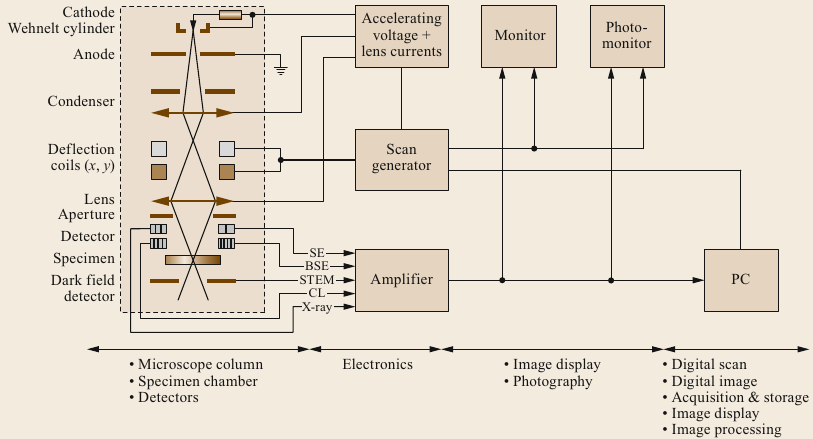
\includegraphics[width=\textwidth]{img/sem_schematic}
    \caption{
    Schematische Darstellung eines konventionellen SEM.
    Die evakuierte Mikroskopsäule (im gestrichelten Rahmen) beinhaltet die Elektronenkanone, elektromagnetische Linsen, Blenden, Probenebene und Detektoren. \cite{springer-handbook}
    }
    \label{fig:sem_schematic}
\end{figure}

Im Folgenden soll der Fokus auf Sekundärelektronen und rückgestreute Elektronen gelegt werden.
Sekundärelektronen sind dadurch definiert, dass sie eine Energie von weniger als \SI{50}{eV} haben, während rückgestreute Elektronen darüber liegen.

Rückgestreute Elektronen werden zu einem kleinen Teil dadurch erklärt, dass ein kleiner Teil der Primärelektronen mit hohem Streuwinkel $\theta > \SI{90}{\degree}$ in Richtung Elektronenkanone zurückgestreut werden und dabei wenig bis keine Energie verlieren.
Da solche Streuprozesse jedoch relativ unwahrscheinlich sind, spielen im BSE-Signal Elektronen, die nach mehreren elastischen Streuprozessen die Probe verlassen die größere Rolle.
Je nach Probeneigenschaften und Primärenergie ergibt sich eine maximale Austrittstiefe, aus der Elektronen nachgewiesen werden können.
Üblicherweise befinden sich BSE-Detektoren auf einer Seite der Elektronenkanone, sodass vornehmlich Elektronen, die in diese Richtung austreten, detektiert werden.
Da dies bei Oberflächen, die dem Detektor zugewandt sind, wahrscheinlicher ist, ergibt sich ein oberflächenorientierungsabhängiges Signal, das mit einem Schattenwurf in Lichtbildaufnahmen vergleichbar ist.
Außerdem nimmt die Wahrscheinlichkeit, dass Elektronen rückgestreut werden, mit der Ladungszahl zu, sodass BSE-Bilder chemischen Kontrast zeigen können (vgl. \cref{fig:bse-schatten}).

\begin{figure}[!ht]
    \centering
    \begin{subfigure}{0.505\textwidth}
        \centering
        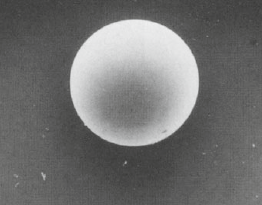
\includegraphics[width=\textwidth]{img/se-example}
    \caption{SE}
    \end{subfigure}
    %\hfill
    \begin{subfigure}{0.3\textwidth}
        \centering
        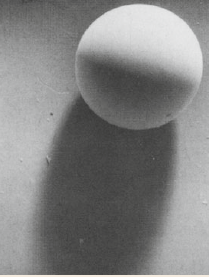
\includegraphics[width=\textwidth]{img/bse-example}
        \caption{BSE}
    \end{subfigure}
    \caption{
     SE- und BSE-Aufnahme einer \SI{1}{mm} großen Stahlkugel. \cite{springer-handbook}
    }
    \label{fig:bse-schatten}
\end{figure}

Sekundärelektronen entstehen durch inelastische Streuung hochenergetischer Elektronen mit Probenatomen.
Hierbei wird Energie auf Elektronen in der Probe übertragen, welche aus ihrem Atompotenzial gelöst werden und danach die Energiedifferenz zwischen übertragener Energie und Ionisationsenergie als kinetische Energie besitzen.
Ist die kinetische Energie ausreichend groß und findet die Ionisation ausreichend nah an der Probenoberfläche statt, kann das Elektron die Probe verlassen und nachgewiesen werden. %2nm
Flächen, die nicht senkrecht zum Primärstrahl stehen, begünstigen die Austrittswahrscheinlichkeit, wodurch SE-Bilder Informationen über die Topographie der Probe beinhalten.

Der Detektor kann sowohl das Objektivlinsensystem des Primärstrahls nutzen (through-the-lens detection) und somit parallel zum Primärstrahl messen oder seitlich montiert sein, wobei ebenfalls ein virtueller Schattenwurf erzeugt wird. \cite{springer-handbook}
In beidem Fällen wird ein Spannungsgradient verwendet, um möglichst viele Elektronen \enquote{einzusammeln}.

\subsection{Probenpräparation für SEM}
%sample preperation requirements: vakuum, conductive for sem, thin for tem etc.
%Leitfähigkeit

Zunächst einmal ist es wichtig, dass dicke Proben (z.B. ganze Insekten) mit einer leitenden Schicht (üblicherweise Gold) beschichtet werden, um elektrostatische Aufladungen der untersuchten Stelle zu verhindern.

Des Weiteren stellt sich bei biologischen Proben das Problem, dass, damit diese in die Vakuumkammer eingebracht werden können, das Wasser aus der Probe entfernt werden muss.
Passierte dies nicht, würde die Probe ins Vakuum ausgasen.
Da Trocknung an der Luft häufig zu einer Zerstörung der zu untersuchenden Strukturen führt, gibt es Methoden, die Struktur der Probe während der Fixierung möglichst gut zu erhalten.

Die Methode der chemischen Fixierung verwendet verschiedene Chemikalien (u.a. Glutaraldehyd, Formaldehyd und Acrolein), um Verbindungen zwischen Aminosäuren, Proteinen und Lipiden herzustellen (üblicherweise durch kovalente Bindungen). \cite{bitesize}
Diese Chemikalien werden in einer Pufferlösung (isotonische Trägerflüssigkeit) eingebracht, um so die Morphologie der Probe zu erhalten.
Um dann das Wasser aus der Probe zu verdrängen, wird dieses zuerst langsam durch Ethanol (oder Aceton) ersetzt und dann in einer Druckkammer durch flüssiges CO$^2$.
Der Zwischenschritt über Ethanol ist nötig, da sich CO$^2$ nicht mit Wasser lösen lässt.
Dann wird ausgenutzt, dass der kritische Punkt von CO$^2$ in einer Druckkammer erreicht werden kann und hier eine Trocknung ohne Verdampung möglich ist, sodass feinporöse Strukturen nicht zerstört werden.

Da biologische Proben größtenteils aus leichten Elementen bestehen, ist in der Regel Absorption, elastische und inelastische Streuung gering, weshalb der Einsatz von Kontrastmitteln (z.B. Osmium(VIII)-oxid) nötig ist.
Diese bringen schwere Elemente (Blei, Uran, Osmium) in die Probe ein, die sich an unterschiedlichen Strukturen besser oder schlechter anlagern, und können hier als letzter Schritt aufgebracht werden.

Als Alternative zur chemischen Fixierung kann die Cryo-Fixierung genannt werden, die auf eine chemische Behandlung der Probe verzichtet, aber ein speziell dafür ausgerüstetes SEM benötigt.
Hier wird auf ein so schnelles Einfrieren der Probe gesetzt, dass keine Eiskristalle entstehen können, welche die Probenstruktur (zer-)stören könnten.

%Chemische Fixierung:
% Fixation
% Chem. Fixation
% Dehydration (ethanol, acetone)
%exchange of acetone with pressurized liquid co2
%kritisch-Punkt-Trocknung
%coating (contrast)
% SEM

%vermutlich egal, weil nicht gemacht, vielleicht nur erwähnen, dass es existiert; Vorteil=no chemical treatment:
% Cryo-Fixierung:
% Fixation
% Cryo-Fixation
% freeze-fracturing
% partial freeze-drying
% coating (contrast)
% Cryo-SEM



\subsection{TEM}

Transmissionselektronenmikroskopie (TEM) erlaubt aufgrund der geringen Wellenlänge hochenergetischer Elektronen, Auflösungen zu erreichen, die mit Lichtmikroskopie aufgrund des Abbe-Limits unmöglich sind.
So kann mittels STEM (scanning transmission electron microscopy) in kristallinen Proben subatomare Auflösung, also die Visualisierung einzelner Orbitale, erreicht werden.
Auch in biologischen Proben können mittels TEM Strukturen beobachtet werden, die im Lichtmikroskop nicht zugänglich sind.
Als Bild ergibt sich so auf dem Leuchtschirm eine Abbildung der Probe, in der für Elektronen schlecht durchlässige Bereiche dunkler als durchlässigere Bereiche erscheinen.
Im Allgemeinen sind Elemente höherer Ordnungszahl schlechter durchlässig.
%Wenn der Typ STEM, Dunkelfeld gemacht hat oder sonst irgendwas spezielles, sollte ich das erwähnen, aber hat er nicht.

\subsection{Probenpräparation für TEM}
%sample preperation requirements: vakuum, conductive for sem, thin for tem etc.

Ähnlich wie in der SEM lassen sich auch hier vor allem zwei Methoden unterscheiden.

In der chemischen Methode wird zunächst Wasser in der Probe durch Aceton ersetzt.
Dann wird das Lösemittel graduell durch ein Harz ersetzt, welches die Probe aushärtet. \cite{bitesize}
Mittels eines speziellen Messers werden dann dünne Scheiben von der Probe abgetrennt und auf TEM-Netze transferiert.
Dies ist nowendig, da TEM im Gegensatz zu SEM extrem dünn geschnittene Proben erfordert, damit ausreichend viele Elektronen die Probe durchqueren, um ein Signal zu messen.
Auch hier werden Kontrastmittel, die schwere Elemente beinhalten, aufgetragen.
% Aufbringen auf Tem-Netze

Die andere Methode ist die Cryo-Fixierung, wobei mit einer gefrorenen Probe angefangen wird, die während des Einbringens des Harzes langsam aufgetaut wird.
Dieser Prozess dauert mehrere Tage bis zu Wochen.

%Chemische Fixierung:
% 1. Fixation
% 2. Dehydration
% 3. Embedding
% 4. Thin sectioning
% 5. Staining (uranyl-acetate, lead-cytrate)

%Cryo-Fixierung
% analog, außer am anfang gefroren und ca. während embedding aufgetaut, takes days-weeks

\subsection{Astigmatismus}

Astigmatismus tritt sowohl im TEM als auch im SEM auf, wenn Elektronen in unterschiedlichen Bildrichtungen eine unterschiedliche Fokusebene haben.
Astigmatismus entsteht durch Herrstellungsfehler in den Polstücken der Linsen.
Ein hoher Astigmatismus sorgt für eine Verzerrung oder Unschärfe des Bildes in einer Bildrichtung. \cite{MyScope}
Korrigieren lässt sich Astigmatismus durch Stigmatoren (Oktupole) in Kondensator- und Objektivlinsen, mithilfe deren man ein Feld aufbaut, das diese Herrstellungsfehler ausgleicht.

%\section{Durchführung}

%actual sample preperation


%TEM:
%schwarze Punkte: schwere Elemente (OsO4 die ja vorher für Kontrast da reingepackt wurden).
	%sO4 gibt Kontraste für Lipide.
	%r mehr Kontraste: Urandingens, etc. => differential staining, differential contrast

	\section{SEM}

% ~5 Bilder
% tif-Dateien: je 2 Bilder, eins bse, eins se
% Vergrößerung im Bild ist manchmal falsch. auf die im Dateinahmen achten. aber die scale bar ist eh ausreichend
% what have we seen: charging artefacts (bad sample coating/high magnification, charge buildup)
%bse/se difference (bse gives composition: heavy elements),
%piece of insect antenna: auflösungslimit, astigmatismuskorrektu wird während Bildaufnahme geändert=>Streifen im Bild
%Insektenaugen: rechts implodiert, links nicht



In \cref{fig:insekt_implosion} ist die Sekundärelektronenaufnahme eines Insektenkopfs bei unterschiedlichen Vergrößerungen dargestellt.
Es ist deutlich zu erkennen, dass hier eine erhebliche Beschädigung des Probenobjekts durch den Trocknungsprozess vorliegt.
Dadurch, dass das Insekt an Atmosphärenluft getrocknet ist, sind die Facetten der Augen implodiert.
Zum Vergleich ist in \cref{fig:mottenauge} die Aufnahme eines Mottenauges abgebildet, bei dem eine solche Implosion trotz Lufttrocknung nicht vorliegt.



\begin{figure}[!ht]
    \centering
    \begin{subfigure}{0.465\textwidth}
        \centering
        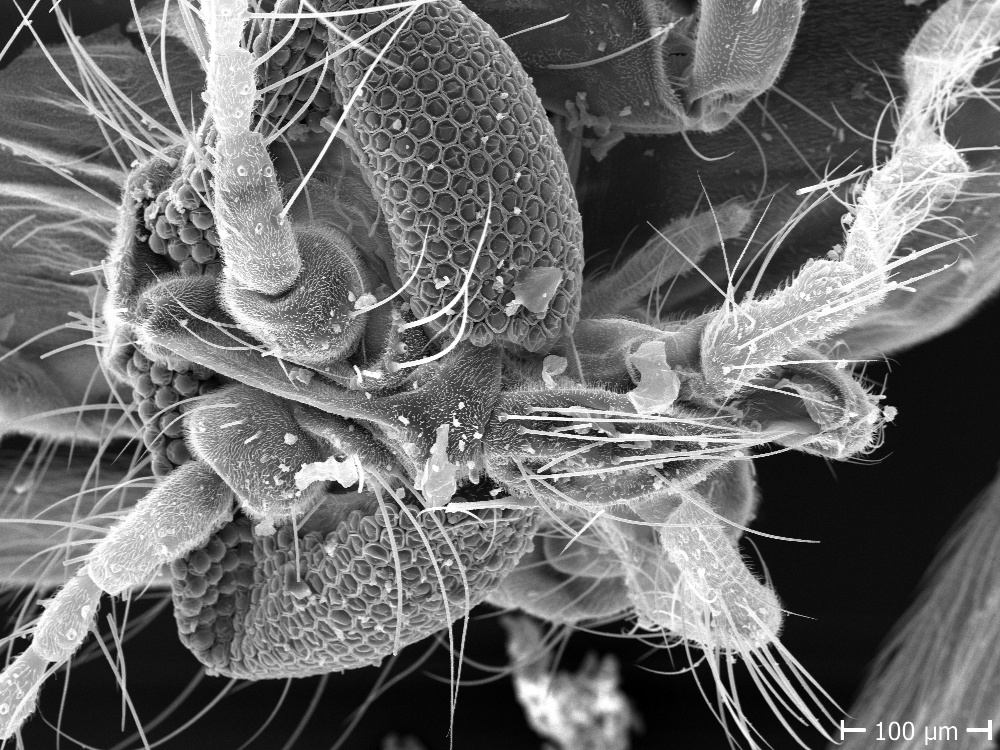
\includegraphics[width=1.1\textwidth]{img/SEM/10.9.20 9_08_08_Mag_ 180x_SE_insect_.jpg}
    \caption{}
    \end{subfigure}
    \hfill
    \begin{subfigure}{0.465\textwidth}
        \centering
        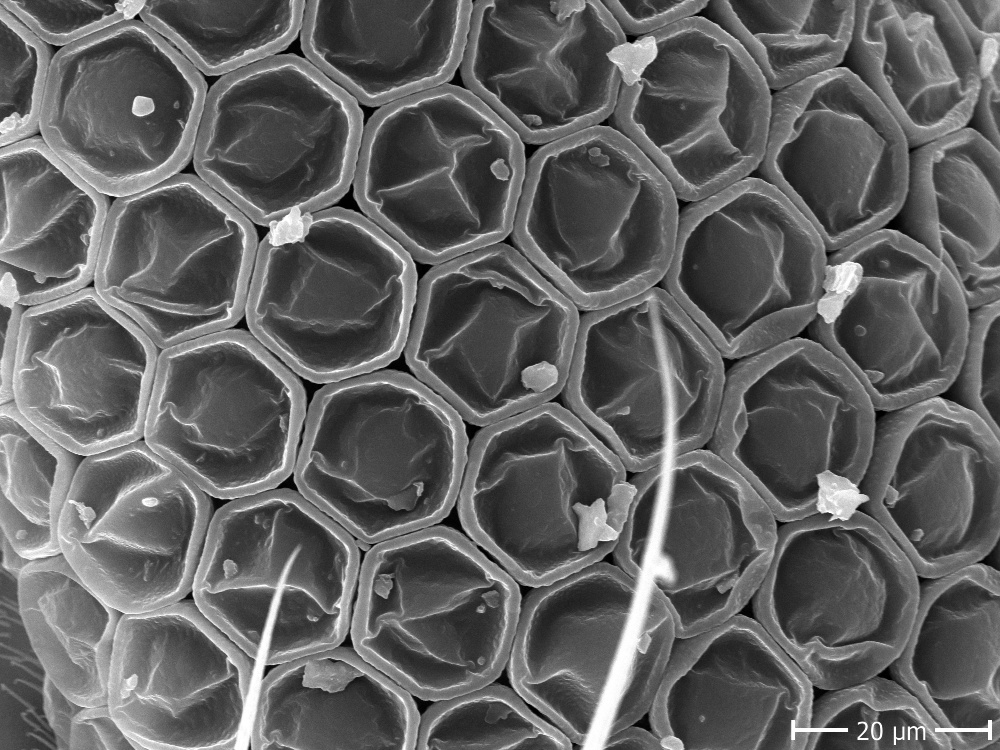
\includegraphics[width=1.1\textwidth]{img/SEM/10.9.20 9_11_43_Mag_ 1200x_SE_insect_eye_drying_artififact.jpg}
        \caption{}
    \end{subfigure}
    \caption{Sekundärelektronenaufnahmen eines luftgetrockneten Insektenkopfs bei unterschiedlichen Vergrößerungen.}
      \label{fig:insekt_implosion}
\end{figure}

\begin{figure}[!ht]
    \centering
    \begin{subfigure}{0.465\textwidth}
        \centering
        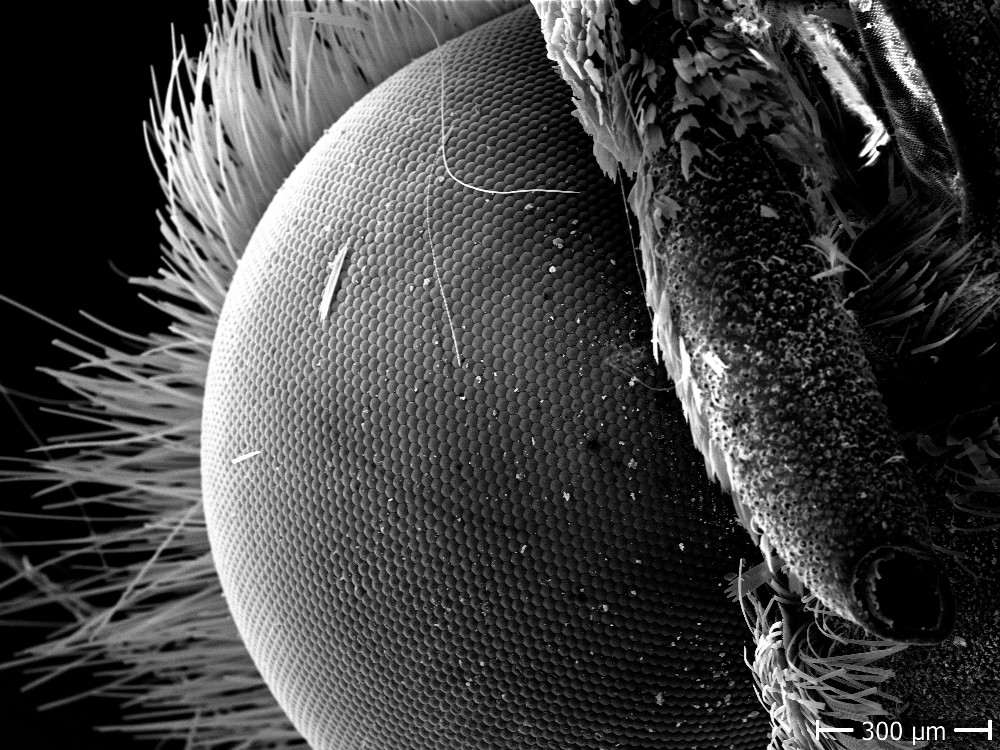
\includegraphics[width=1.1\textwidth]{img/SEM/10.9.20 9_44_08_Mag_ 70x_SE_moth_eye}
    \caption{}
    \end{subfigure}
    \hfill
    \begin{subfigure}{0.465\textwidth}
        \centering
        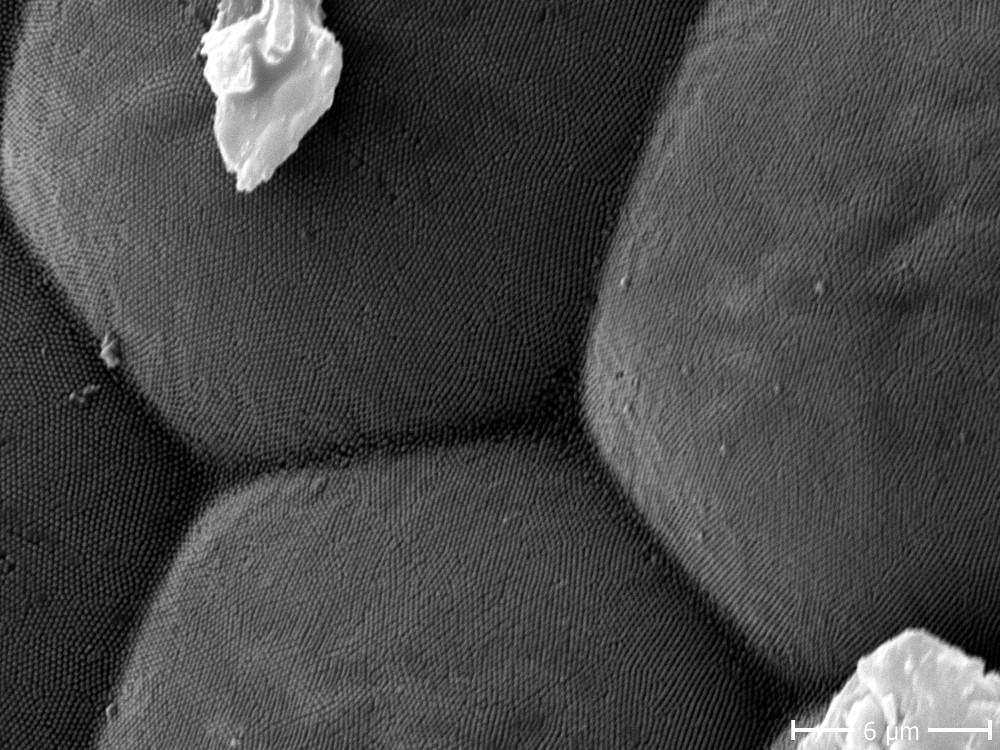
\includegraphics[width=1.1\textwidth]{img/SEM/10.9.20 9_46_35_Mag_ 4000x_SE_moth_eye}
        \caption{}
    \end{subfigure}
    \caption{Sekundärelektronenaufnahmen eines luftgetrockneten Mottenauges bei unterschiedlichen Vergrößerungen.}
      \label{fig:mottenauge}
\end{figure}

In der Aufnahme einer Insektenantenne in \cref{fig:astigmatenne} wurde während des Scans die Astigmatismuskorrektur geändert.
Dies drückt sich im Bild anhand von horizontalen Streifen aus.

\begin{figure}[!ht]
    \centering
    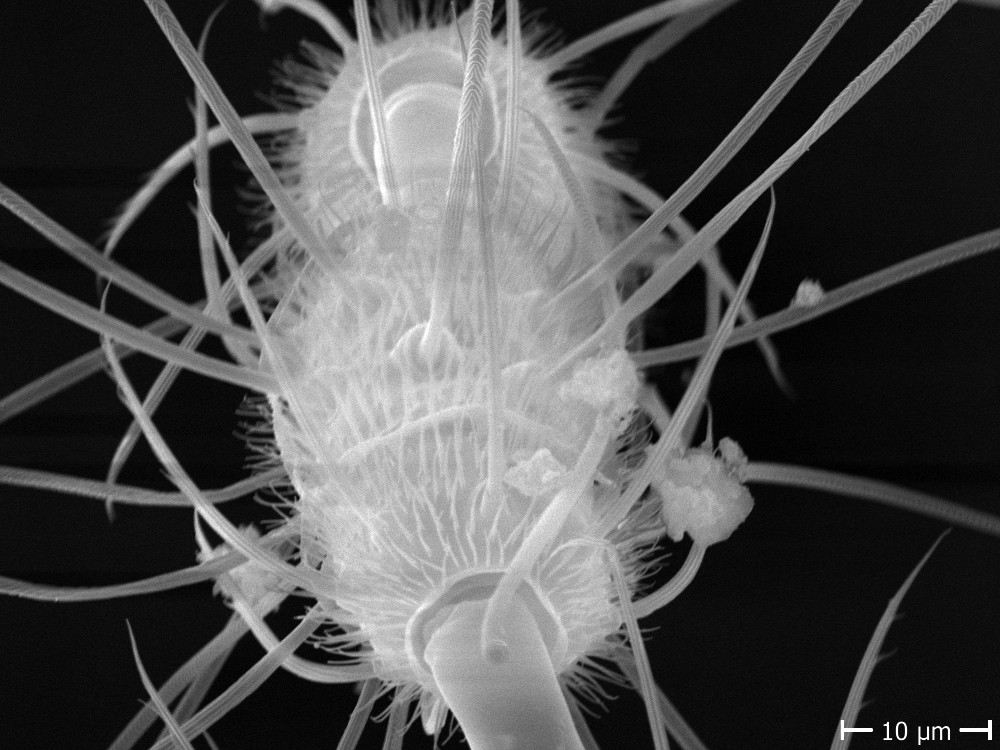
\includegraphics[width=0.65\textwidth]{img/SEM/10.9.20 11_09_41_Mag_ 1800x_astigmatism_introduced}
    \caption{Sekundärelektronenaufnahme der Antenne eines Insekts. Während der Aufnahme wurde die Astigmatismuskorrektur geändert.}
    \label{fig:astigmatenne}
\end{figure}

	\section{TEM}

% ~5 Bilder
% what have we seen: charging artefacts (bad sample coating/high magnification, charge buildup)

%artefakte: kleine runde Wassereinschlüsse in der Plastikbeschichtung => Loch in der Probe
%schwarze streifen: irgendwelche Fehler in der Beschichtung
%schwarze Punkte: schwere Elemente (OsO4 die ja vorher für Kontrast da reingepackt wurden).
	%sO4 gibt Kontraste für Lipide.
	%r mehr Kontraste: Urandingens, etc. => differential staining, differential contrast
	%robe wurde nicht richtig abgewaschen => Kristalle dieser Salze als Kontamination auf der Oberfläche
%bild mit Gitter: kondensierte dna (nucleoli,) und Helferzelle, vat-grown (also zumindest nicht aus echtem Hirn)
%dann Helferzelle.
	%hne Kontrastmittel: auf reine Eiskristalle fokussieren, dann mit der Fokussierung Zytoplasma, Mitochondrien anschauen
	%resnel-(Ränder) um die Mitochondrien durch interferenz. Nucleus ist das große Runde.
%golgi(?)-Apparatus: Zysterny, einmal senkrecht, einmal parallel geschnischnitten
%im tem ist damage durch e-beam. runde helle fläche war in voriger vergrößerung fokussiert.
%Muskeln: quergestreifte Muskeln. Eine Zelle om menschl. Bizeps ist 15cm lang (Schulter bis ellenbogen), 1 Mikrometer abstand haben die schwarzen linien (Scheiben da dings)
	%ote Blutzelle oben links. bringt Glukose zu zelle, mitochondrien (Kreise) wandeln in ATP um=> Kontraktion der Mysin-Aktin-Dinger
	%chwarze Linien sind die Scheiben, wo das Aktin dranhängt und Myosin jeweils dazwischen
%irgendwas mit Platin: Platin in tiefen deposited (i think), "platinum replicas", sem-like image durch Invertierung
	%das Platin ist halt so als Form irgendwo die Topografie abgepauscht

In \cref{fig:tem:waben} ist eine TEM-Aufnahme bei geringer Vergrößerung zu sehen.
Deutlich sichtbar ist die Wabenstruktur des TEM-Netzes und ein Loch in der Probe, das durch Wassereinschlüsse in der Plastikbeschichtung entstanden ist. %TODO welcher Schritt der Präparation?

\begin{figure}[!ht]
    \centering
    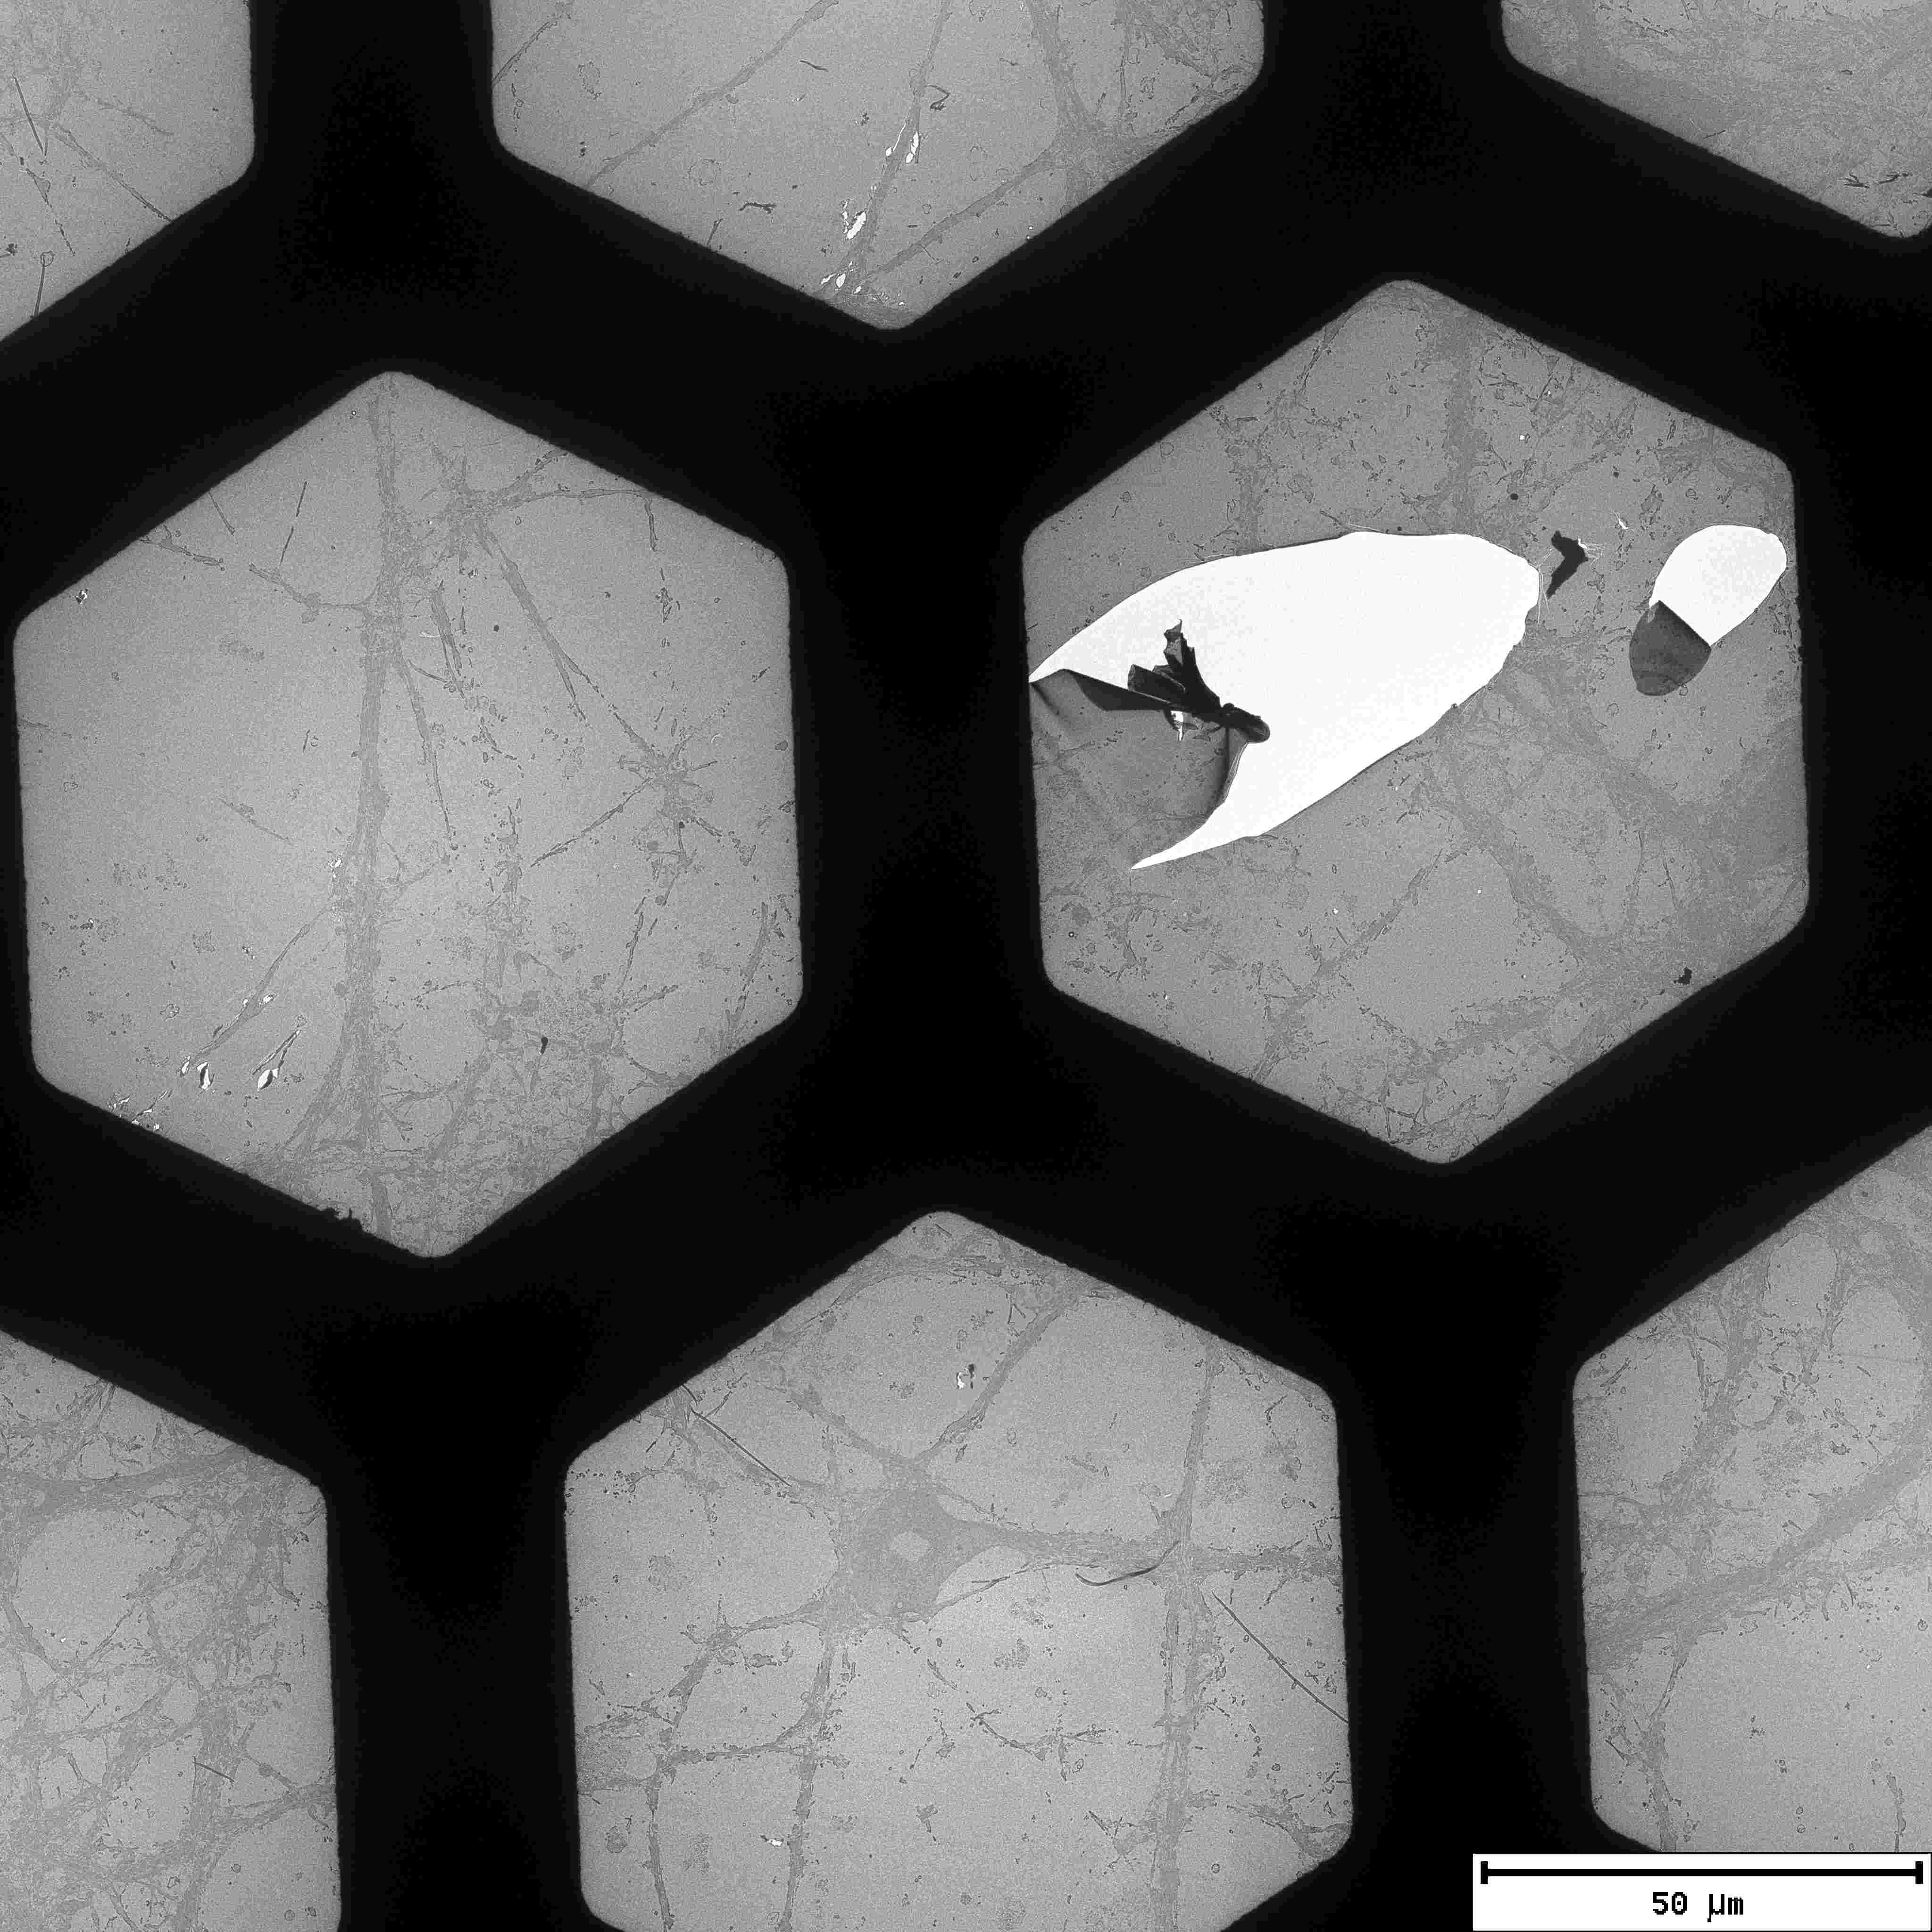
\includegraphics[width=0.65\textwidth]{img/TEM/1_low_mag_artifacts.jpg}
    \caption{TEM-Lichtbildaufnahme von kondensierter DNA (Nucleoli) und Helferzellen, in-vitro gewachsen, bei geringer Vergrößerung.} %TODO hoffentlich ist das tatsächlich die Probe
    \label{fig:tem:waben}
\end{figure}

In \cref{fig:tem:ahk} ist die Aufnahme eines Astrozyten dargestellt.
Es sind Eiskristalle sichtbar, welche durch Fehler beim Abwaschen der Probe entstehen, wobei Salzkontaminationen auf der Oberfläche zurückgeblieben sind.
Dabei wurde zunächst auf die Eiskristalle fokussiert, wodurch um die Mitochondrien Fresnel-Ränder (Interferenzeffekt bei Objekten vor oder hinter der Fokusebene) sichtbar werden.

\begin{figure}[!ht]
    \centering
    \includegraphics[width=0.65\textwidth]{img/TEM/2_astrocyte_house_keeper.jpg}
    \caption{TEM-Lichtbildaufnahme einer Astrozyten-Helferzelle im unteren linken Viertel des Bildes. Fokussiert wurde auf die Eiskristalle im oberen rechten Bildbereich.}
    \label{fig:tem:ahk}
\end{figure}

	\newpage
\section{Schlussfolgerung}
	% Rückgriff auf Hypothese und drittes Nennen dieser
	% Quellen zitieren, Websiten mit Zugriffsdatum
	% Verweise auf das Laborbuch (sind erlaubt)
	% Tabelle + Bilder mit Beschriftung

  Zusammenfassend lässt sich sagen, dass 

		% --- Anhang einbinden
	%\newpage
\appendix
\newpage
\section{Anhang}\label{sec:anhang}

%\subsection{Unsicherheiten}\label{sec:unsicherheiten}

Alle Unsicherheiten werden nach dem GUM bestimmt und berechnet.
Die Gleichungen dazu finden sich in \ref{fig:GUM_combine} und \ref{fig:GUM_formula}.
Hierfür wurde die Python Bibliothek \enquote{uncertainties} verwendet, welche den Richtlinien des GUM folgt.
Für die Unsicherheiten der Parameter in Annäherungskurven wurden die $y$-Unsicherheiten der anzunähernden Werte beachtet und die Methode der kleinsten Quadrate angewandt.
Dafür steht in der Bibliothek die Methode \enquote{scipy.optimize.curve\_fit()} zur Verfügung.

Für Messungen mit digitalen Anzeigen wird eine rechteckige Verteilung mit $\sigma_X = \frac{\Delta X}{2\sqrt{3}}$ aufgrund der begrenzten Ziffernzahl und für analoges Ablesen wird eine Dreiecksverteilung mit $\sigma_X = \frac{\Delta X}{2\sqrt{6}}$ angenommen.
Die jeweiligen $\Delta X$ sind im entsprechenden Abschnitt zu finden.

\begin{figure}[ht]
	\begin{equation*}
	x = \sum_{i=1}^{N} x_i
	;\quad
	\sigma_x = \sqrt{\sum_{i = 1}^{N} \sigma_{x_i}^2}
	\end{equation*}
	\caption{Formel für kombinierte Unsicherheiten des selben Typs nach GUM.}
	\label{fig:GUM_combine}
\end{figure}

\begin{figure}[ht]
	\begin{align*}
	f = f(x_1, \dots , x_N)
	;\quad
	\sigma_f = \sqrt{\sum_{i = 1}^{N}\left(\pdv{f}{x_i} \sigma_{x_i}\right) ^2}
	\end{align*}
	\caption{Formel für sich fortpflanzende Unsicherheiten erster Ordnung nach GUM.}
	\label{fig:GUM_formula}
\end{figure}

\begin{table}[H]
	\centering
	\caption{Ergebnisse aus den Fits ausgewählter Peaks in den Massenspektren. MVM meint Matrix, Verdünnungsstufe ($\log_{10}(c \cdot \si{\liter \per \mole})$) und Modus des Flugzeitspektrometers (HR/S). SRV ist das Signal-Rausch-Verhältnis.}
	\resizebox{\textwidth}{!}{%
	\begin{tabular}{c | c | c | c | c}
MVM & Position ($m/z$) & Halbwertsbreite & Massenauflösung $R$ & SRV \\ \hline
DHB-7S	& \SI{ 734.57044 \pm 0.00023 }{} & \SI{ 0.0563 \pm 0.0006 }{} & \SI{ 1.304 \pm 0.013e+04 }{} & \SI{ 101 \pm 27 }{}\\
	& \SI{ 760.58588 \pm 0.00021 }{} & \SI{ 0.0596 \pm 0.0005 }{} & \SI{ 1.277 \pm 0.011e+04 }{} & \SI{ 90 \pm 19 }{}\\
DHB-7S	& \SI{ 734.57001 \pm 0.00020 }{} & \SI{ 0.0560 \pm 0.0005 }{} & \SI{ 1.312 \pm 0.012e+04 }{} & \SI{ 85 \pm 17 }{}\\
	& \SI{ 760.58550 \pm 0.00026 }{} & \SI{ 0.0612 \pm 0.0007 }{} & \SI{ 1.243 \pm 0.013e+04 }{} & \SI{ 51 \pm 7 }{}\\
DHB-6S	& \SI{ 734.5691 \pm 0.0007 }{} & \SI{ 0.0602 \pm 0.0017 }{} & \SI{ 1.219 \pm 0.035e+04 }{} & \SI{ 17.2 \pm 2.1 }{}\\
	& \SI{ 760.5853 \pm 0.0006 }{} & \SI{ 0.0626 \pm 0.0016 }{} & \SI{ 1.214 \pm 0.032e+04 }{} & \SI{ 21.3 \pm 3.0 }{}\\
DHB-5S	& \SI{ 734.57021 \pm 0.00023 }{} & \SI{ 0.0566 \pm 0.0006 }{} & \SI{ 1.298 \pm 0.013e+04 }{} & \SI{ 81 \pm 17 }{}\\
	& \SI{ 760.58573 \pm 0.00025 }{} & \SI{ 0.0580 \pm 0.0006 }{} & \SI{ 1.312 \pm 0.015e+04 }{} & \SI{ 108 \pm 33 }{}\\
CHCA-5S	& \SI{ 734.57025 \pm 0.00024 }{} & \SI{ 0.0553 \pm 0.0006 }{} & \SI{ 1.329 \pm 0.015e+04 }{} & \SI{ 65 \pm 12 }{}\\
	& \SI{ 760.58590 \pm 0.00022 }{} & \SI{ 0.0601 \pm 0.0006 }{} & \SI{ 1.266 \pm 0.012e+04 }{} & \SI{ 74 \pm 13 }{}\\
DHB-4HR	& \SI{ 734.56227 \pm 0.00018 }{} & \SI{ 0.0217 \pm 0.0004 }{} & \SI{ 3.39 \pm 0.07e+04 }{} & \SI{ 1.0 \pm 0.5e+02 }{}\\
	& \SI{ 760.5789 \pm 0.0004 }{} & \SI{ 0.0212 \pm 0.0009 }{} & \SI{ 3.58 \pm 0.16e+04 }{} & \SI{ 1.6 \pm 2.4e+02 }{}\\
DHBA-4S	& \SI{ 734.56961 \pm 0.00022 }{} & \SI{ 0.0485 \pm 0.0005 }{} & \SI{ 1.516 \pm 0.017e+04 }{} & \SI{ 1.4 \pm 0.5e+02 }{}\\
	& \SI{ 760.58515 \pm 0.00022 }{} & \SI{ 0.0504 \pm 0.0006 }{} & \SI{ 1.509 \pm 0.017e+04 }{} & \SI{ 1.4 \pm 0.5e+02 }{}\\
	& \SI{ 734.56547 \pm 0.00008 }{} & \SI{ 0.01889 \pm 0.00021 }{} & \SI{ 3.89 \pm 0.04e+04 }{} & \SI{ 1.9 \pm 0.6e+02 }{}\\
	& \SI{ 760.58107 \pm 0.00011 }{} & \SI{ 0.01993 \pm 0.00026 }{} & \SI{ 3.82 \pm 0.05e+04 }{} & \SI{ 3.1 \pm 2.0e+02 }{}\\
DHB-4H	& \SI{ 734.56532 \pm 0.00009 }{} & \SI{ 0.01984 \pm 0.00023 }{} & \SI{ 3.70 \pm 0.04e+04 }{} & \SI{ 1.8 \pm 0.6e+02 }{}\\
	& \SI{ 760.58040 \pm 0.00030 }{} & \SI{ 0.0211 \pm 0.0008 }{} & \SI{ 3.61 \pm 0.13e+04 }{} & \SI{ 1.6 \pm 2.9e+02 }{}\\
DHB-4S	& \SI{ 734.56939 \pm 0.00020 }{} & \SI{ 0.0508 \pm 0.0005 }{} & \SI{ 1.445 \pm 0.014e+04 }{} & \SI{ 1.5 \pm 0.5e+02 }{}\\
	& \SI{ 760.58470 \pm 0.00021 }{} & \SI{ 0.0515 \pm 0.0005 }{} & \SI{ 1.477 \pm 0.015e+04 }{} & \SI{ 1.4 \pm 0.5e+02 }{}\\
DHB-4S	& \SI{ 734.56954 \pm 0.00023 }{} & \SI{ 0.0513 \pm 0.0006 }{} & \SI{ 1.433 \pm 0.016e+04 }{} & \SI{ 1.3 \pm 0.4e+02 }{}\\
	& \SI{ 760.58489 \pm 0.00020 }{} & \SI{ 0.0542 \pm 0.0005 }{} & \SI{ 1.404 \pm 0.013e+04 }{} & \SI{ 1.5 \pm 0.5e+02 }{}\\
CHCA-4HR	& \SI{ 734.56593 \pm 0.00027 }{} & \SI{ 0.0183 \pm 0.0007 }{} & \SI{ 4.02 \pm 0.15e+04 }{} & \SI{ 1.2 \pm 1.1e+02 }{}\\
	& \SI{ 760.58217 \pm 0.00014 }{} & \SI{ 0.01832 \pm 0.00034 }{} & \SI{ 4.15 \pm 0.08e+04 }{} & \SI{ 2.3 \pm 2.0e+02 }{}\\
CHC-4S	& \SI{ 734.56831 \pm 0.00018 }{} & \SI{ 0.0576 \pm 0.0005 }{} & \SI{ 1.276 \pm 0.010e+04 }{} & \SI{ 113 \pm 26 }{}\\
	& \SI{ 760.58334 \pm 0.00018 }{} & \SI{ 0.0605 \pm 0.0005 }{} & \SI{ 1.257 \pm 0.010e+04 }{} & \SI{ 1.5 \pm 0.4e+02 }{}\\
CHCA-4HR	& \SI{ 734.56643 \pm 0.00018 }{} & \SI{ 0.0188 \pm 0.0004 }{} & \SI{ 3.91 \pm 0.09e+04 }{} & \SI{ 83 \pm 30 }{}\\
	& \SI{ 760.58104 \pm 0.00021 }{} & \SI{ 0.0203 \pm 0.0005 }{} & \SI{ 3.75 \pm 0.09e+04 }{} & \SI{ 2.6 \pm 3.0e+02 }{}\\
	& \SI{ 734.5637 \pm 0.0004 }{} & \SI{ 0.0183 \pm 0.0009 }{} & \SI{ 4.02 \pm 0.20e+04 }{} & \SI{ 1.0 \pm 0.9e+02 }{}\\
	& \SI{ 760.58013 \pm 0.00025 }{} & \SI{ 0.0209 \pm 0.0006 }{} & \SI{ 3.64 \pm 0.11e+04 }{} & \SI{ 2.5 \pm 3.1e+02 }{}\\
CHCA-4S	& \SI{ 734.56806 \pm 0.00024 }{} & \SI{ 0.0579 \pm 0.0006 }{} & \SI{ 1.268 \pm 0.013e+04 }{} & \SI{ 108 \pm 31 }{}\\
	& \SI{ 760.58363 \pm 0.00021 }{} & \SI{ 0.0585 \pm 0.0005 }{} & \SI{ 1.301 \pm 0.012e+04 }{} & \SI{ 121 \pm 35 }{}\\
	\end{tabular}
	}
	\label{tab:massiv}
\end{table}

		
	\printbibliography


\end{document}
